\section{Experiments}\label{sec:exp}
\subsection{Implementation Details}
% Source: configs/lecun-deliver_rgbdel_P46_c3only_seed20260821_screen40_A2hires.yaml (TRAIN, OPTIMIZER, SCHEDULER, LOSS, MODEL.M2F, MODEL.P46.C3_PROTO, MODEL.P39).
All sensors are converted to three-channel images as in CMNeXt~\cite{cmnext2023}. We train for 40 epochs with AdamW (learning rate $6\times10^{-4}$, weight decay 0.01), a polynomial schedule with power 0.9, and a 10-epoch warm-up, on $768\times768$ crops with an effective batch size of 16 obtained by gradient accumulation. We use the data augmentation of DGFusion~\cite{dgfusion2026} so that both models see the same augmented images. The clean-pass loss combines online hard-example cross-entropy~\cite{ohem2016} on the final logits with the set-prediction loss of the query head (weight 0.5, with deep supervision), the auxiliary sensor heads (0.5), the router (cross-entropy 0.4 and regularizer 0.01), a class-prototype contrastive term (0.1), and a variance-covariance regularizer on the per-sensor tokens (variance weight 0.1 and covariance weight 0.01, scaled by 1.0 for LiDAR and 0.25 for the other sensors). These terms are inherited from earlier versions of our model; we list them for reproducibility and do not ablate them. The frozen teacher is the same architecture without the high-resolution path, trained for 200 epochs on clean data. All results of our model are the mean of three training runs with different seeds, unless a table states otherwise; the leave-one-out ablation in Table~\ref{tab:ablation_loo} uses one seed.

\subsection{Comparison with Prior Fusion Models}
Table~\ref{tab:deliver} compares \ours{} with fusion models on DELIVER. Part~(a) lists methods with a reported test-split result, which is the split we compare on; part~(b) lists methods that report only validation results, which come from different training and evaluation settings and are shown for completeness. \ours{} reaches 57.74 test mIoU, 1.0 point above the published DGFusion result (56.7). Its margin over MM SAM-adapter, which uses only RGB and depth, is 0.4 points (our three-seed mean). On the validation set, \ours{} scores 70.17 on average, 1.6 points above CAFuser-CAA (68.6); StitchFusion with a Swin-T backbone reports 70.3 without naming the split, so our validation result is not the highest published one. Tables~\ref{tab:muses} and~\ref{tab:mcubes} report the same model on the real MUSES and MCubeS benchmarks \todo{results pending: MUSES four-sensor model, MCubeS transfer}.
% Sources: headline.yaml deliver.ours[0] (57.74 = 3-seed mean; best seed 58.61 is recorded in notes/table_sources.md, not shown: user 2026-11-02). Published DGFusion test = 56.7 (DGFusion Table III p6, notes/sota_survey.md):
%   gap +1.04 (text rounds to 1.0). CAFuser-CAA val 68.6 (CAFuser Table III p6) -> +1.57.
%   68.79 (old draft) has no source and was removed (sota_survey.md 0). StitchFusion Swin-T 70.3: StitchFusion Table 1 p6.
% protocol clusters: repo research/novelty-and-related-work.md l.74-85 (secondary; cite original tables).


% Layout rule (user 2026-10-27): no \resizebox on tables. Every table uses \tabsetup and
% tabular* at \columnwidth, so all tables share one font size and none overflows the column.

% ---------------------------------------------------------------------------
% Table 1. DELIVER, all four sensors.
% Baselines: only the test-unified cluster (DGFusion protocol, "mIoU-test").
%   Do NOT mix with the high cluster (CMNeXt 66.30 / MemorySAM 65.38).
%   Candidate values for todo cells are in repo research/novelty-and-related-work.md:78-83
%   (secondary copy) -> must be taken from each original paper table, cite table+page.
% Ours: experiments/headline.yaml benchmarks.deliver.ours[0] (A2, 3 seeds, legal v2, test@1024).
%   val 3-seed mean 70.17 = tasks/DRN-261019-03 report R03:23.
% ---------------------------------------------------------------------------
\begin{table}[t]
\caption{Comparison with fusion methods on DELIVER (mIoU, \%). Results of other methods are taken from the cited papers.}
\label{tab:deliver}
\centering\tabsetup
\begin{tabular*}{\columnwidth}{@{\extracolsep{\fill}}lllcc@{}}
\toprule
Method & Backbone & Sensors & val & test \\
\midrule
\multicolumn{5}{@{}l}{\emph{(a) All four sensors, test split reported}} \\
CMNeXt~\cite{cmnext2023}$^{a}$ & MiT-B2 & RGB-D-E-L & 66.3 & 53.0 \\
StitchFusion~\cite{stitchfusion2024}$^{a}$ & MiT-B2 & RGB-D-E-L & 68.2 & 53.4 \\
GeminiFusion~\cite{geminifusion2024}$^{a}$ & MiT-B2 & RGB-D-E-L & 66.9 & 54.5 \\
CAFuser-CAA~\cite{cafuser2025} & Swin-T & RGB-D-E-L & 68.6 & 55.2 \\
CAFuser~\cite{cafuser2025} & Swin-T & RGB-D-E-L & 67.8 & 55.6 \\
DGFusion~\cite{dgfusion2026} & Swin-T & RGB-D-E-L & -- & 56.7 \\
\midrule
\multicolumn{5}{@{}l}{\emph{(b) All four sensors, validation split only}} \\
MemorySAM~\cite{memorysam2025}$^{b}$ & Hiera-B+ & RGB-D-E-L & 65.38 & -- \\
MLE-SAM~\cite{mlesam}$^{b}$ & Hiera-B+ & RGB-D-E-L & 64.08 & -- \\
OmniSegmentor~\cite{omnisegmentor2025}$^{b}$ & MiT-B2 & RGB-D-E-L & 67.5 & -- \\
OmniSegmentor~\cite{omnisegmentor2025}$^{b}$ & DFormer-L & RGB-D-E-L & 68.0 & -- \\
HyperDUM~\cite{hyperdum2025} & MiT-B2 & RGB-D-E-L & 67.59 & -- \\
MAGIC~\cite{magic2024} & MiT-B2 & RGB-D-E-L & 67.66 & -- \\
Any2Seg~\cite{any2seg2024} & MiT-B2 & RGB-D-E-L & 68.25 & -- \\
FuseAdapt~\cite{fuseadapt2026}$^{b}$ & DINOv2-B & RGB-D-E-L & 68.33 & -- \\
StitchFusion~\cite{stitchfusion2024}$^{b}$ & Swin-T & RGB-D-E-L & \best{70.3} & -- \\
\midrule
\multicolumn{5}{@{}l}{\emph{(c) Fewer sensors}} \\
MM SAM-adapter~\cite{mmsamadapter2025} & SAM ViT-L & RGB-E & 60.74 & 55.70 \\
MM SAM-adapter~\cite{mmsamadapter2025} & SAM ViT-L & RGB-L & 61.89 & 57.14 \\
MM SAM-adapter~\cite{mmsamadapter2025} & SAM ViT-L & RGB-D & 69.60 & \second{57.35} \\
\midrule
Ours & DINOv3-L & RGB-D-E-L & \second{70.17} & \best{57.74} \\
\bottomrule
\end{tabular*}
\tabnote{$^{a}$Both values as listed by CAFuser~\cite{cafuser2025} (Table~III); the test values were measured by the CAFuser authors. $^{b}$The source does not name the split; listed as validation because it is compared there against validation results. Validation results come from different training and evaluation settings and are not directly comparable. Ours: mean of three seeds.}
\end{table}

% ---------------------------------------------------------------------------
% Table 2. MUSES, four sensors (RGB, event, LiDAR, radar). Only the 4-sensor A2 model
%   (user 2026-09-29; 3-sensor numbers 79.788 etc. are not used).
% Ours: DRN-261019-02 (queued) -> todo. Baselines: headline.yaml benchmarks.muses.
% ---------------------------------------------------------------------------
\begin{table}[t]
\caption{Comparison with fusion methods on MUSES (mIoU, \%). Test results are from the official evaluation server, as reported in the cited papers.}
\label{tab:muses}
\centering\tabsetup
\begin{tabular*}{\columnwidth}{@{\extracolsep{\fill}}lllcc@{}}
\toprule
Method & Backbone & Sensors & val & test \\
\midrule
\multicolumn{5}{@{}l}{\emph{(a) Camera only}~\cite{muses2024}} \\
Mask2Former~\cite{mask2former2022} & Swin-T & RGB & -- & 70.7 \\
SegFormer~\cite{segformer2021} & MiT-B2 & RGB & -- & 72.5 \\
SegFormer~\cite{segformer2021} & MiT-B5 & RGB & -- & 74.7 \\
Mask2Former~\cite{mask2former2022} & Swin-L & RGB & -- & 77.1 \\
\midrule
\multicolumn{5}{@{}l}{\emph{(b) Four sensors}} \\
CMNeXt~\cite{cmnext2023}$^{a}$ & MiT-B2 & RGB-L-R-E & -- & 72.4 \\
GeminiFusion~\cite{geminifusion2024}$^{a}$ & MiT-B2 & RGB-L-R-E & -- & 75.3 \\
CAFuser~\cite{cafuser2025} & Swin-T & RGB-L-R-E & -- & 78.2 \\
CAFuser-CAA~\cite{cafuser2025} & Swin-T & RGB-L-R-E & -- & 78.5 \\
DGFusion~\cite{dgfusion2026} & Swin-T & RGB-L-R-E & -- & 79.5 \\
\midrule
\multicolumn{5}{@{}l}{\emph{(c) Fewer sensors}} \\
FuseAdapt~\cite{fuseadapt2026} & DINOv2-S & RGB-L-E & 77.28 & -- \\
MM SAM-adapter~\cite{mmsamadapter2025} & SAM ViT-L & RGB-E & -- & \second{79.92} \\
MM SAM-adapter~\cite{mmsamadapter2025} & SAM ViT-L & RGB-L & -- & \best{81.07} \\
\midrule
Ours & DINOv3-L & RGB-L-R-E & \td & \td \\
\bottomrule
\end{tabular*}
\tabnote{R: radar. $^{a}$As measured by the CAFuser authors~\cite{cafuser2025} (Table~II).}
\end{table}

% ---------------------------------------------------------------------------
% Table 3. MCubeS (RGB, AoLP, DoLP, NIR). Ours: DRN-261017-02 (A2 transfer, 2 seeds) -> todo.
%   58.07 in headline.yaml is the previous generation (P39.1 recipe), not the paper model.
% ---------------------------------------------------------------------------
\begin{table}[t]
\caption{Comparison on the MCubeS test set with RGB, AoLP, DoLP, and NIR inputs (mIoU, \%).}
\label{tab:mcubes}
\centering\tabsetup
\begin{tabular*}{\columnwidth}{@{\extracolsep{\fill}}lllc@{}}
\toprule
Method & Backbone & Sensors & test \\
\midrule
MCubeSNet~\cite{mcubes2022} & ResNet-101 & RGB-A-D-N & 42.86 \\
ShareCMP~\cite{sharecmp2023} & MiT-B2 & RGB-A-D & 50.99 \\
MLE-SAM~\cite{mlesam} & Hiera-B+ & RGB-A-D-N & 51.02 \\
CMNeXt~\cite{cmnext2023} & MiT-B2 & RGB-A-D-N & 51.54 \\
U3M~\cite{u3m2024} & SegFormer & RGB-A-D-N & 51.69 \\
Any2Seg~\cite{any2seg2024} & MiT-B2 & RGB-A-D-N & 51.91 \\
Cao et al.~\cite{bpcf2026} & MiT-B4 & RGB-A-D-N & 52.22 \\
StitchFusion~\cite{stitchfusion2024} & Swin-T & RGB-A-D-N & 52.3 \\
MemorySAM~\cite{memorysam2025} & Hiera-B+ & RGB-A-D-N & 52.88 \\
MAGIC~\cite{magic2024} & MiT-B2 & RGB-A-D-N & 53.01 \\
MMSFormer~\cite{mmsformer2023} & MiT & RGB-A-D-N & 53.11 \\
StitchFusion~\cite{stitchfusion2024} & MiT-B4 & RGB-A-D-N & 53.92 \\
StitchFusion~\cite{stitchfusion2024} & Swin-L & RGB-A-D-N & \second{55.9} \\
FuseAdapt~\cite{fuseadapt2026} & DINOv2-B & RGB-A-D-N & \best{57.62} \\
\midrule
Ours & DINOv3-L & RGB-A-D-N & \td \\
\bottomrule
\end{tabular*}
\tabnote{A: AoLP, D: DoLP, N: NIR.}
\end{table}

\subsection{Robustness to Missing and Degraded Sensors}
Table~\ref{tab:robust} evaluates robustness with the benchmark of~\cite{mmssbench2025} on the DELIVER validation set. To compare under identical conditions, we run the public evaluation code of the benchmark on our model and on the baselines whose code and weights are public, and list only such methods. \todo{numbers of \ours{} and of the baselines in (b) under the benchmark code (analysis request, 2026-11-04); the earlier measurement with our own scorer (native-resolution labels, no flip) gave EMM 57.85, RMM 61.28--65.53 and NM 58.34/51.92/39.99 and is kept only in the notes until the re-measurement}.
% Sources: tasks/DRN-261019-03/analysis.md (val clean 70.17, EMM15 57.85, RMM 65.53/63.35/61.28); 2503.18445 Tables 3, 7-11;
% drop clean-EMM: ours 70.17-57.85 = 12.32; benchmark models 66.33-37.90 = 28.43 ... 68.20-41.98 = 26.22, MAGIC 66.10-44.97 = 21.13.
% Removed 2026-11-02 (user): test-split S&P-only noise numbers and the DGFusion test EMM sentences (kept in judgment-ledger).
% judgment-ledger:130 DRN-261001-03 (official weights clean 56.73, EMM 31.14, NM drop 52.20 -> 4.53);
% judgment-ledger:117 (reproduction (a) EMM 31.53, NM .20 5.52; retrained (b) EMM 45.52); current.md (4) CAFuser (b) EMM 46.50;
% MAGIC 44.97: arXiv 2503.18445 Table 7 (mIoU_EMM^Avg, MiT-B2, val).

When only one sensor is available (Fig.~\ref{fig:robust}b), the released DGFusion weights collapse to 7.5 mIoU with RGB alone and to 1.1 with event or LiDAR alone, while still reaching 43.3 with depth alone. Training with degraded inputs lifts every single-sensor score, most strongly for RGB (49.0 for the re-trained DGFusion and 53.9 for our model without the high-resolution path).
% Sources: judgment-ledger:130 (official weights single-sensor 7.50/43.33/1.13/1.13); judgment-ledger:117 (retrained 49.0/44.5/25.0/25.0; Q2 3 seeds 53.9/46.0/31.0/22.9).

% ---------------------------------------------------------------------------
% Table 5. Missing and noisy sensors on DELIVER val under the benchmark of arXiv 2503.18445 (user 2026-11-02:
% the paper uses this benchmark; channel-shared salt-and-pepper-only numbers were removed).
% (a) arXiv 2503.18445 (MiT-B2): clean = Table 3 RDEL column; EMM Avg and E(p) = Table 7; RMM Avg r=.75/.5/.25 =
%     Tables 8/9/10; NM Low/Mid/High = Table 11 (mIoU_NM row). Read from the PDF text (notes/missing_bench_survey.md).
% (b) Methods published after the benchmark with the same definition: notes/missing_bench_survey.md (2026-11-02).
%     [removed 2026-11-04, user: open methods only; no public code found] EQUISeg = arXiv 2509.24505 Table 1 p4 (DeLiVER: mIoU 67.90, EMM Avg 48.22, EMM p=0.1 65.75, RMM Avg 50.96,
%     RMM p=0.1 64.64, NM Low 34.87, Mid 19.13); its baseline rows equal 2503.18445 Table 9 (r=0.5) -> RMM column r=.50.
%     RMMSS = 2505.12861 Table 2 p6 (MiT-B0, EMM 49.93, RMM 51.90, r not stated) -> footnote only.
% (c) Baselines measured by us with tools/missing_modality_eval.py on val: analysis inbox 20261102-180010 (pending).
% Fairness check 2026-11-04: benchmark val_mm_NM.py (github Chenfei-Liao/Multi-Modal-Semantic-Segmentation-Robustness-Benchmark)
%   injects S&P (tensor max/min) then Gaussian (RGB, D, L) on the normalized batch from get_val_augmentation; CMNeXt
%   Normalize = ImageNet for img, /255 for others; ours identical (NORM_ALL_MODALS off in configs/eval/a2s821_eval1024_hpca100_probe.yaml).
%   Benchmark NM script evaluates with sliding_predict(flip=True); ours without TTA.
% (d) Ours (A2, 3 seeds): tasks/DRN-261019-03/analysis.md val clean 70.17, EMM15 57.85, RMM r.25/.5/.75
%     65.53/63.35/61.28. NM (DRN-261102-04, nm_mode bench, val) = mean of hpca100 ~/SSDb/jemo_maeng/nmbench_20261102/
%     s821/s902/s903_val/val/missing_modality/summary.json (md5 f98fb583 / 46f6fa86 / 153b8e3b): Low 57.84/59.29/57.88,
%     Mid 51.52/52.79/51.45, High 39.63/40.21/40.12 -> 58.34 / 51.92 / 39.99 (clean in the same files 69.59/71.05/69.86).
%     E(p): inbox 20261102-180010 (seed 903 only so far: 66.10/68.20/69.09).
% ---------------------------------------------------------------------------
\begin{table*}[t]
\caption{Robustness to missing and noisy sensors on the DELIVER validation set under the benchmark protocol of~\cite{mmssbench2025} (mIoU, \%).}
\label{tab:robust}
\centering\tabsetup
\begin{tabular*}{\textwidth}{@{\extracolsep{\fill}}llccccccccccc@{}}
\toprule
 & & & \multicolumn{4}{c}{Entire-missing (EMM)} & \multicolumn{3}{c}{Random-missing (RMM), Avg} & \multicolumn{3}{c}{Noisy (NM)} \\
\cmidrule(lr){4-7}\cmidrule(lr){8-10}\cmidrule(l){11-13}
Method & Backbone & Clean & Avg & E(.20) & E(.10) & E(.05) & $r$=.75 & $r$=.50 & $r$=.25 & Low & Mid & High \\
\midrule
\multicolumn{13}{@{}l}{\emph{(a) Reported by the benchmark~\cite{mmssbench2025}}} \\
CMNeXt~\cite{cmnext2023} & MiT-B2 & 66.33 & 37.90 & 54.46 & 60.41 & 63.38 & 42.17 & 47.49 & \second{53.61} & \best{35.23} & 16.37 & 2.31 \\
GeminiFusion~\cite{geminifusion2024} & MiT-B2 & 66.92 & 37.07 & 54.33 & 60.62 & 63.77 & 39.78 & 42.41 & 49.74 & 5.52 & 4.14 & 3.30 \\
MAGIC~\cite{magic2024} & MiT-B2 & 66.10 & \best{44.97} & \second{58.66} & 62.68 & 64.47 & \second{45.30} & 48.19 & 51.61 & 24.03 & 13.31 & 3.98 \\
MAGIC++~\cite{magicpp2024} & MiT-B2 & \second{67.34} & \second{44.85} & \best{59.18} & \best{63.52} & \second{65.50} & \best{47.06} & \best{49.31} & \best{53.92} & \second{33.12} & \best{18.31} & \second{8.70} \\
StitchFusion~\cite{stitchfusion2024} & MiT-B2 & \best{68.20} & 41.98 & 58.02 & \second{63.29} & \best{65.80} & 45.16 & \second{48.33} & 53.10 & 24.91 & \second{17.11} & \best{9.25} \\
\midrule
\multicolumn{13}{@{}l}{\emph{(b) Evaluated by us with the benchmark code}} \\
DGFusion$^{\ast}$ & Swin-T & \td & \td & \td & \td & \td & \td & \td & \td & \td & \td & \td \\
DGFusion (retrained$^{\dagger}$) & Swin-T & \td & \td & \td & \td & \td & \td & \td & \td & \td & \td & \td \\
CAFuser (retrained$^{\dagger}$) & Swin-T & \td & \td & \td & \td & \td & \td & \td & \td & \td & \td & \td \\
\midrule
Ours & DINOv3-L & \td & \td & \td & \td & \td & \td & \td & \td & \td & \td & \td \\
\bottomrule
\end{tabular*}
\tabnotewide{Avg: mean over the 15 non-empty sensor subsets; E($p$): expectation when each sensor fails independently with probability $p$; RMM $r$: fraction of a removed sensor's values that are zeroed; NM Low/Mid/High: salt-and-pepper density and Gaussian standard deviation (0.05, 0.1), (0.1, 0.2), (0.2, 0.5). All definitions follow~\cite{mmssbench2025} and Section~\ref{sec:sensors}. All entries are produced with the public evaluation code of the benchmark (single forward pass for EMM and RMM, horizontal-flip averaging for NM, labels resized with the input to $1024\times1024$); only methods with public code and weights are listed. $^{\ast}$Released weights. $^{\dagger}$Retrained with synthetic degradation and modality dropout, without distillation. Ours: mean of three seeds; baselines: single runs. Methods that skip a missing input instead of zero-filling it answer a different question and are not listed.}
\end{table*}

% ---------------------------------------------------------------------------
% Fig. robust (data plot). Source numbers and provenance: figures/src/make_data_figs.py (fig_robust).
% ---------------------------------------------------------------------------
\begin{figure}[t]
\centering
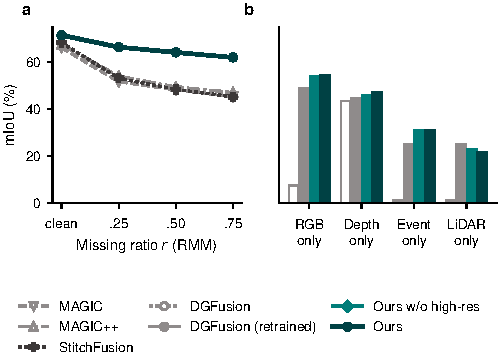
\includegraphics[width=\columnwidth]{figures/fig_robust.pdf}
\caption{Robustness on DELIVER. (a) Random-missing sensors on the validation set: mIoU averaged over the 15 sensor subsets as the missing ratio $r$ grows. Benchmark models (MiT-B2) are taken from~\cite{mmssbench2025}; our curves use our own scorer. (b) A single available sensor on the test set, with the other three zero-filled. Ours: mean of three seeds; baselines: single runs. \todo{(a) our curves: re-measure with the benchmark code; (b) full-model values pending.}}
\label{fig:robust}
\end{figure}

\subsection{Qualitative Results}
Figs.~\ref{fig:failure_scenarios} and~\ref{fig:adverse} show scenes selected by a fixed rule: among all test images, those where the gap between our model and the best of the other models is largest, with no two scenes from the same sequence. With all sensors present (Fig.~\ref{fig:adverse}), this gap is 3.4 to 5.9 points of per-image mIoU on the six scenes shown (2.9 to 5.9 points over the 18 scenes of Appendix~\ref{app:qual}), while the opposite selection, the scene of each condition where another model leads ours the most (Fig.~\ref{fig:reverse}), gives gaps of 8.4 to 10.1 points; per-image differences are therefore modest in both directions when every sensor works \todo{describe the visible error regions; sensor-failure scenes (Fig.~\ref{fig:failure_scenarios}) pending}.

% Fig. sensor-failure scenarios (main qualitative figure). Needs per-image predictions of
% DGFusion (official), DGFusion/CAFuser (retrained) and ours under missing/noisy sensors
% -> analysis request inbox 20261027-182054 item 2.
\begin{figure*}[t]
\centering
\phbox{5.2cm}{Fig.~3 when a sensor fails: rows = depth missing / RGB missing / LiDAR+event missing / RGB with heavy noise; columns = affected input, ground truth, CMNeXt, CAFuser, DGFusion, ours; error pixels in one colour}
\caption{Qualitative comparison on the DELIVER test set when a sensor fails. Rows: depth missing, RGB missing, LiDAR and event missing, and RGB with heavy noise. Columns: affected input, ground truth, CMNeXt, CAFuser, DGFusion, and ours. Each row shows the scene where ours most exceeds the best other method in per-image mIoU, with no repeated sequence.}
\label{fig:failure_scenarios}
\end{figure*}

% Fig. adverse conditions with all sensors present, DELIVER (synthetic) + MUSES (real).
% DELIVER dumps exist: NAS analysis_logs/native_axis_baseline_20261016/{dgfusion,cafuserb}_test1024,
% a2_test1024_dump_20261016/s821 -> analysis request inbox 20261027-182054 item 1. MUSES: item 3.
\begin{figure*}[p]
\centering
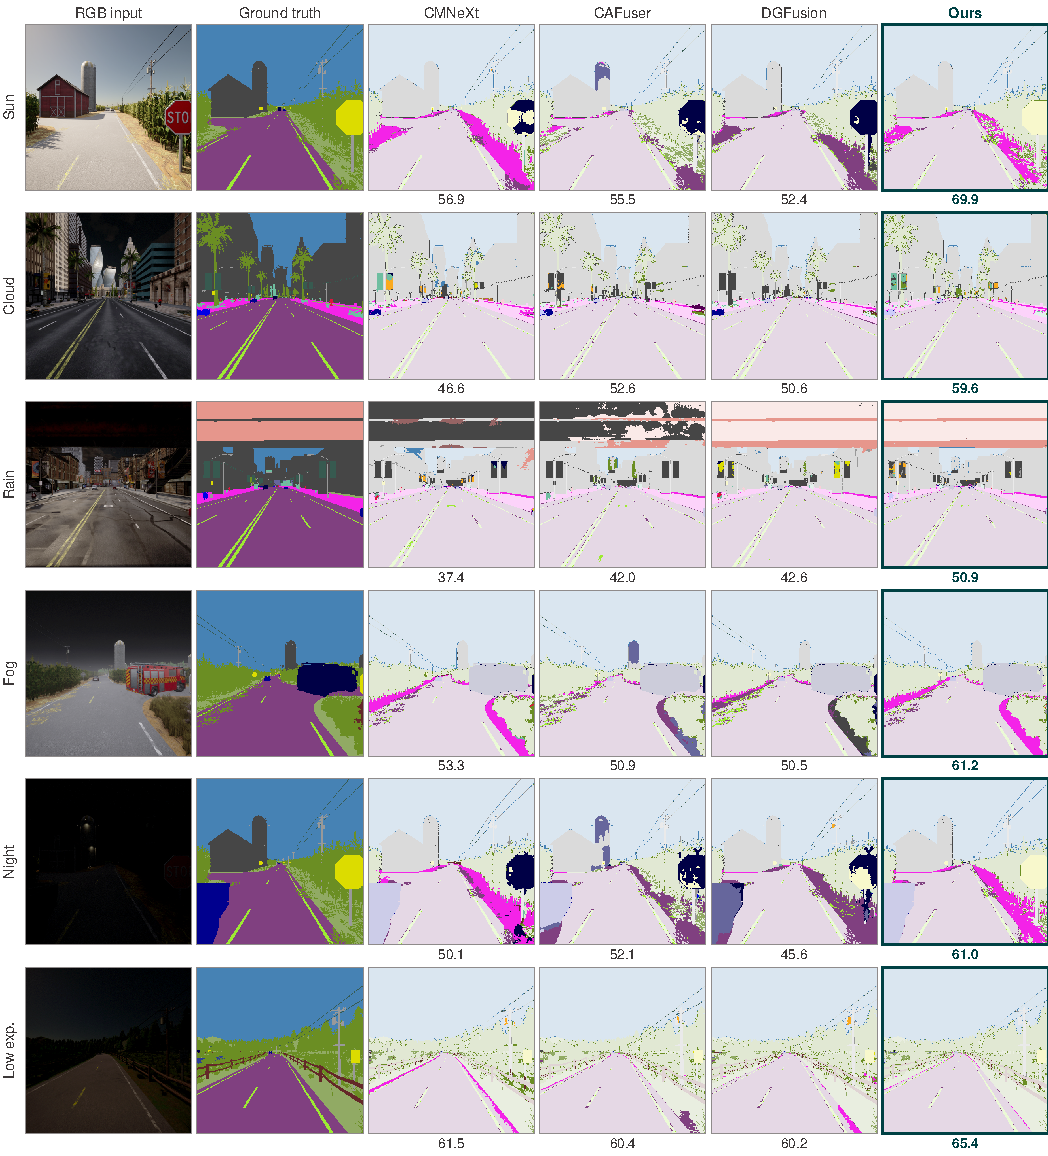
\includegraphics[width=\textwidth]{figures/fig_adverse_deliver.pdf}\\[3pt]
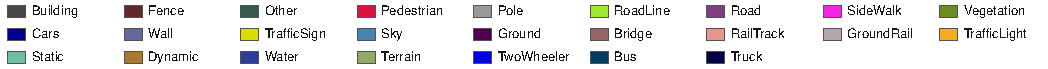
\includegraphics[width=\textwidth]{figures/fig_class_legend_deliver.pdf}
\caption{Qualitative comparison on the DELIVER test set under six conditions with all four sensors. Columns: RGB input, ground truth, CMNeXt, CAFuser, and DGFusion (released weights), and ours. Each row shows the scene where ours most exceeds the best of the other three methods in per-image mIoU, with no two scenes from the same sequence. Faded pixels agree with the ground truth, so colored pixels are errors; numbers give per-image mIoU (\%). More scenes are in Appendix~\ref{app:qual}. \todo{tiles are regenerated when the CMNeXt and CAFuser dumps arrive}}
\label{fig:adverse}
\end{figure*}

% Fig. MUSES real adverse conditions (same layout as fig:adverse; analysis inbox 20261030-122055 P2).
\begin{figure*}[t]
\centering
\phbox{4.6cm}{MUSES val, all sensors: real night / snow / fog / rain; columns = RGB, ground truth, CMNeXt, CAFuser, DGFusion, ours (released weights, release order); same selection rule; waits for the MUSES 4-sensor model}
\caption{\todo{MUSES counterpart of Fig.~\ref{fig:adverse}; same rule on the 250 validation images (test labels are not public)}}
\label{fig:adverse_muses}
\end{figure*}

\subsection{Accuracy per Condition}
Table~\ref{tab:condition} breaks clean test accuracy down by condition \todo{text after the per-condition numbers arrive (analysis request 20261028-183826 item 1)}.

% ---------------------------------------------------------------------------
% Table 5. Clean mIoU per condition on DELIVER test (new 2026-10-28).
% Source: to be computed by analysis from the same dumps as Fig. adverse (inbox addendum).
% ---------------------------------------------------------------------------
\begin{table}[t]
\caption{Per-condition results on the DELIVER test set with all four sensors (mIoU, \%).}
\label{tab:condition}
\centering\tabsetup
\begin{tabular*}{\columnwidth}{@{\extracolsep{\fill}}lccccccc@{}}
\toprule
Model & Sun & Cloud & Rain & Fog & Night & Low exp. & All \\
\midrule
DGFusion$^{\ast}$ & \td & \td & \td & \td & \td & \td & \second{56.73} \\
DGFusion (retrained$^{\dagger}$) & \td & \td & \td & \td & \td & \td & 54.77 \\
CAFuser (retrained$^{\dagger}$) & \td & \td & \td & \td & \td & \td & 55.79 \\
Ours & \td & \td & \td & \td & \td & \td & \best{57.74} \\
\bottomrule
\end{tabular*}
\tabnote{$^{\ast}$Released weights. $^{\dagger}$Retrained with synthetic degradation and modality dropout, without distillation. All: test mIoU over all conditions from the same measurement as the other columns.}
\end{table}

\subsection{Ablation}
Table~\ref{tab:abl_robust} measures the two additions, the C2D2 training scheme and the high-resolution path, over three seeds, and Table~\ref{tab:ablation_loo} removes one component at a time from the full model with one seed. A frozen DINOv3-L with LoRA on RGB alone already reaches 55.14 mIoU on the test set (one seed), within 1.6 points of DGFusion with four sensors, so a large part of the accuracy comes from the foundation model. On the test set, the high-resolution path raises mIoU from 56.59 to 57.74 \todo{effect of C2D2 alone: three-seed test mean of the clean-trained model}. Removing cross-modal attention costs 0.85 points. \todo{the degradation-pass and distillation rows (L5, L6) pending}.
% Sources: judgment-ledger 2026-10-28 rows DRN-261020-08/-09/-10/-12 (seed 821, legal v2 test@1024);
% E1 screen s821 55.94: status/current.md (4); Q2/A2 s821 57.73/58.61: tasks/DRN-261019-03/analysis.md.

% ---------------------------------------------------------------------------
% Table 6. Ablation on DELIVER test, seed 821, 40 epochs, legal v2.
% RGB-only 55.14 = judgment-ledger 2026-10-28 DRN-261020-08 (adopted as ladder row).
% L2 mean fusion 57.76 = judgment-ledger 2026-10-28 (L4 dense head only 57.89 removed from the paper: user 2026-11-04, query-head ablation dropped)
%   rows DRN-261020-09/-10/-12 (test@1024 legal v2, seed 821). L2 also removes the trunk expansion
%   (code constraint, ledger note). L5 DRN-261020-13 / L6 -14 evaluating; mean-fusion ladder -07 running.
% mean fusion = DRN-261020-07 (evaluating). E1 screen s821 55.94 = status/current.md (4).
% Q2 s821 57.73 / EMM 48.68 and A2 s821 58.61 / EMM 49.12 = tasks/DRN-261019-03/analysis.md.
% Leave-one-out: L2 DRN-261020-10, L4 -12, L5 -13, L6 -14, L7 DRN-261029-01. L3 withdrawn. L1 (one adapter for all sensors) is
% excluded from this paper (user 2026-11-02, inbox 20261102-191138) and kept for the separate RA-L paper.
% ---------------------------------------------------------------------------
% Table "incremental ablation" (tab:ablation) removed 2026-11-04 (user): its C2D2 / high-res rows duplicated tab:abl_robust.

% Table 6b. Leave one component out of the full model (one seed, 40 epochs). Sources as Table 6 comment above;
% L5 DRN-261020-13 (evaluating), L6 -14 (judging), L7 DRN-261029-01 (running) -> todo until verdicts.
\begin{table}[t]
\caption{Leave-one-out ablation on the DELIVER test set (mIoU, \%). Each row removes one component from the full model (last row).}
\label{tab:ablation_loo}
\centering\tabsetup
\begin{tabular*}{\columnwidth}{@{\extracolsep{\fill}}cccccc@{}}
\toprule
Cross- & Degr. & Phys. & Teacher & Clean & EMM \\
modal & pass & degr. & KD & & \\
\midrule
\cmark & \xmark & \xmark & \cmark & \td & \td \\
\cmark & \cmark & \cmark & \xmark & \td & \td \\
\cmark & \cmark & \xmark & \cmark & \td & \td \\
\xmark$^{*}$ & \cmark & \cmark & \cmark & \second{57.76} & \td \\
\cmark & \cmark & \cmark & \cmark & \best{58.61} & 49.12 \\
\bottomrule
\end{tabular*}
\tabnote{All rows keep the high-resolution path. Degr.\ pass: the second, degraded forward pass of the C2D2 scheme. Phys.\ degr.: sensor-specific degradations (blur, exposure, depth holes, beam drop, event down-sampling) instead of zero-filling only, with the same missing-sensor rate. Teacher KD: the distillation term on the degraded pass. $^{*}$Token averaging; also removes the sensor-specific residual $m_s$ of Eq.~(2).}
\end{table}

% Table 6c. Robustness ablation, 3 seeds, DELIVER val, benchmark protocol (user 2026-11-02).
% w/o high-res = Q2 3 seeds val: tasks/DRN-261019-03/analysis.md (clean 67.91, EMM15 56.87, RMM .25/.5/.75 64.08/62.46/60.69).
% w/o C2D2 and high-res (E1 40ep) val: analysis inbox 20261102-180010 (pending).
% w/o C2D2 and high-res = E1 40-ep screen 3 seeds, EMM 40.01 (judgment-ledger 2026-10-01 row);
% w/o high-res = Q2 3 seeds, full = A2 3 seeds: tasks/DRN-261019-03/analysis.md (moved from Table robust (b)).
% MCubeS rows: DRN-261031-01 (w/o C2D2, legal eval pending) and DRN-261017-02 (C2D2, training).
\begin{table}[t]
\caption{Effect of the C2D2 training scheme and the high-resolution path on accuracy and robustness (mIoU, \%, mean of three seeds).}
\label{tab:abl_robust}
\centering\tabsetup
\begin{tabular*}{\columnwidth}{@{\extracolsep{\fill}}cccccccc@{}}
\toprule
C2D2 & High- & Test & \multicolumn{5}{c}{Validation} \\
\cmidrule(l){4-8}
tr. & res & Clean & Clean & EMM & RMM .75 & .50 & .25 \\
\midrule
\multicolumn{8}{@{}l}{\emph{(a) DELIVER, mean of 3 seeds}} \\
\xmark & \xmark & \td & \td & \td & \td & \td & \td \\
\cmark & \xmark & \second{56.59} & \second{67.91} & \second{56.87} & \second{60.69} & \second{62.46} & \second{64.08} \\
\cmark & \cmark & \best{57.74} & \best{70.17} & \best{57.85} & \best{61.28} & \best{63.35} & \best{65.53} \\
\midrule
\multicolumn{8}{@{}l}{\emph{(b) MCubeS}} \\
\xmark & \cmark & \td & & & & & \\
\cmark & \cmark & \td & & & & & \\
\bottomrule
\end{tabular*}
\tabnote{C2D2 tr.: trained with the C2D2 scheme (clean pass, degraded pass, and teacher distillation). Test: test-set mIoU with all sensors. The validation columns of (a) use our own scorer (native-resolution labels, no flip) until the re-measurement with the benchmark code of Table~\ref{tab:robust}; EMM and RMM are averages over the 15 sensor subsets.}
\end{table}

\subsection{Computational Cost}
The C2D2 training scheme changes only how the model is trained: the second, degraded pass and the frozen teacher are used during training and removed afterwards, so the deployed model is the same network with or without this scheme. Its cost therefore comes from the architecture, which Table~\ref{tab:cost} reports at inference. The backbone is frozen, and our model has about as many trainable parameters as the baselines (74.0M against 75.0M and 78.9M). Because every sensor passes through the frozen ViT-L, however, it needs 14.6 times the operations and 2.9 times the latency of DGFusion, about four images per second for four sensors at $1024\times1024$ on one RTX 4090. The high-resolution path adds 15.2M parameters, about 2\% of the operations, and 13\% of the latency. \todo{add the DINOv3-B operating point (DRN-261102-01/-02) to show the accuracy--cost trade-off of a smaller backbone}
% Source: .claude_logs/tasks/DRN-261027-02/analysis.md table (l.14-19), verdict adopt 2026-11-03; raw NAS analysis_logs/cost_table_20261104{,b,c}/.
% Ratios: 10135/695.6 = 14.57; 254.5/88.9 = 2.86; high-res = A2 - Q2: 377.05-361.87 = 15.18M, (10135-9922)/9922 = 2.1%, 254.5/224.8 = 1.13.

% ---------------------------------------------------------------------------
% Table 7. Cost on DELIVER at 1024, same GPU. DRN-261027-02 (adopted; notes/table_sources.md cost rows).
% ---------------------------------------------------------------------------
\begin{table}[t]
\caption{Inference cost on DELIVER with four sensors ($1024\times1024$ input, batch size 1, one RTX 4090, bf16). Trainable: parameters updated during training. The C2D2 training scheme adds no inference cost.}
\label{tab:cost}
\centering\tabsetup
\begin{tabular*}{\columnwidth}{@{\extracolsep{\fill}}lccccc@{}}
\toprule
Model & Params & Trainable & GFLOPs & Latency & Memory \\
 & (M) & (M) & & (ms) & (GB) \\
\midrule
DGFusion~\cite{dgfusion2026} & 78.88 & 78.88 & 695.6 & 88.9 & 1.83 \\
CAFuser~\cite{cafuser2025} & 75.01 & 75.01 & 670.8 & 83.1 & 1.57 \\
Ours & 377.05 & 73.98 & 10{,}135 & 254.5 & 2.47 \\
\bottomrule
\end{tabular*}
\end{table}
